\documentclass[../Languages.tex]{subfiles}

\begin{document}
\usec{Bash}\label{sec:bash}

\cd{Bash} is a Unix shell and command languages written by Brian Fox for the
GNU Project as a free software replacement for the Bourne shell. First released
in 1989, it has been distributed widely as the default login shell for most
Linux distributions and Apple's macOS. A version is also available for Windows
10.

\cd{Bash} is a command processor that typically runs in the text window, where
the user types commands that cause actions. \cd{Bash} can also read and execute
commands from a files, called a script. Like Unix shells, it supports filename
globbing (wildcard matching), piping, here documents, command substitution,
variables, and control structures for condition-testing and iteration. The
keywords, syntax and other basic features of the language are all copied from
\cd{sh}. Other features, e.g., history are copied from \cd{csh}, and \cd{ksh}.
\cd{Bash} is a POSIX-compliant shell, but with a number of extensions.

The shell's name is an acronym for \textit{Bourne-again shell}, punning on the
name of the Bourne shell that it replaces and on the term ``born again'' that
denotes spiritual rebirth in contemporary American Christianity.

A security hole in \cd{Bash} dating from version 1.03, dubbed Shellshock, was
discovered in early September 2014 and quickly led to a range of attacks across
the Internet. Patches to fix the bugs were made available soon after the bugs
were identified, but not all computers have been updated.

\subsection{Influence}
\label{sub:influence}

\begin{Figure}
   \centering
   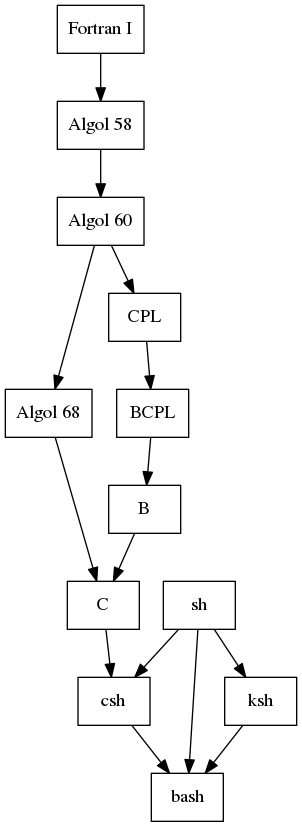
\includegraphics[height=0.5\textheight]{bash}
   \captionof{figure}{Inheritance diagram for \cd{Bash}.}
\end{Figure}

\newpage
\end{document}
